%! Author = aybehrouz



Every transaction in the Argennon blockchain starts with an \texttt{invoke\_external} instruction which calls a
special method from the root smart contract. This method will transfer the proposed fee of the transaction in ARGs
from a sender account to the fee sink accounts. Argennon has two fee sink accounts: \texttt{execFeeSink} collects
execution fees and \texttt{dbFeeSink} collects fees for ZK-EDB servers. The Protocol decides how to distribute the
transaction fee between these two fee sink accounts.

When a block is added to the blockchain, the proposer of that block will receive a share of the block fees.
Consequently, a block proposer is always incentivized to include more transactions in his block. However, if he
puts too many transactions in his block and the validation of the block becomes too difficult, some validators
may not be able to validate all transactions on time. If a validator can not validate a block in the required
time, he will consider the block invalid. So, when a proposed block contains too many transactions, the network
may reach consensus on another block, and the proposer of that block will not receive any fees. As a result, a
proposer is incentivized to use network transaction capacity optimally.

On the other hand, we believe that the proposer does not have enough incentives for optimizing the storage size
of the transaction set. Therefore, we require that \textbf{the size of the transaction set of every block in
bytes be lower than a certain threshold.}

Validators need to spend resources for validating transactions. When a validator starts the emulation of the AVM
to validate a transaction, solely from the code he can't predict the time the execution will finish. This will
give an adversary an opportunity to attack the network by broadcasting transactions that never ends. Since,
validators can not finish the execution of these transactions, the network will not be able to charge the
attacker any fees, and he would be able to waste validators resources for free.

To mitigate this problem, we require that every transaction specify a cap for all the resources it needs. This
will include memory, network and processor related resources. Also, the protocol defines an execution cost for
every AVM instruction reflecting the amount of resources its emulation needs. This will define a standard way for
measuring the execution cost of any \texttt{avmCall} transaction. Every \texttt{avmCall} transaction is required
to specify a maximum execution cost. If during emulation it reaches this maximum cost, the transaction will be
considered failed and the network can receive the proposed fee of that transaction.


In Argennon \emph{light} nodes do not keep a full copy of the AVM storage and for emulating the Argennon Virtual Machine
( i.e.~validating transactions) they need to connect to a ZK-EDB and retrieve the required pages.
Because light node need to be able to validate block certificates, they usually cache a large part of the staking
database, and keep their cache updated to make sure they can keep themselves in sync with the blockchain.


On the other hand, nodes that are chosen to be validators, for validating a new block, need to emulate the
execution of the Argennon Virtual Machine. To do so, first they retrieve all storage pages they
need from available ZK-EDBs. Then, they emulate the execution of AVM instructions and validate all the
transactions included in the new block. This will modify some pages of the AVM storage, so they update the ZK-EDB
commitments based on the modified pages and verify the commitments included in the new block. Validators also
calculate and verify the commitment to the new block's transaction set.

\note{Validators do not need to write the modified pages back to ZK-EDB servers. ZK-EDB servers will receive the new
block, and they will update their database by emulating the AVM execution.}


The only information that all Argennon nodes are required to store is \textbf{the most recent block} of the Argennon
blockchain.
We store the commitment of this
transaction set in every block, but we don't keep the set itself. To be able to detect replay attacks, we require
every signature that a user creates to have a nonce. This nonce consists of the issuance round of the signature
and a sequence number: \texttt{(issuance,\ sequence)}. When a user creates more than one signature in a round, he
must sequence his signatures starting from 0 (i.e.~the sequence number restarts from 0 in every round). We define
a maximum lifetime for signatures, so a signature is invalid if \texttt{currentRound - issuance > maxLifeTime} or
if a signature of the same user with a bigger or equal nonce is already used
(i.e.~is recorded in the blockchain). A nonce is bigger than another nonce if it has an older issuance. If two
nonces have an equal issuance, the nonce with the bigger sequence number will be considered bigger.

To be able to detect invalid signatures, we keep the maximum nonce of used digital signatures per user. When the
difference between \texttt{issuance} component of this nonce and the current round becomes bigger than the
maximum allowed lifetime of a signature, this information can be safely deleted. \textbf{As a result, we will not
have the problem of "un-removable empty accounts" like Ethereum.}



In our system a newly created account will not have voting power for some time, no matter how high its
balance is. While this is a desirable property, in case a large proportion of total system tokens are
transferred to newly created accounts, it can result in too much voting power for older accounts. This may decrease
the degree of decentralization in our system.

However, this situation is easily detectable by comparing the total stake of the system with the total balance of
users. If after confirming a block the total stake of the system goes too low and we have:
\[
    \sum_{u}S_{u,t} < \gamma \sum_{u}B_{u,t}
\]
The protocol will perform a \emph{time shift} in the system: the time step of the system
will be incremented for \(m\) steps while no blocks will be confirmed. This will increase the value of \(M_{u,t}\)
for new accounts with a non-zero balance, giving them more influence in the agreement protocol.

For calculating the value of \(m\) which determines the amount of time shift in the system, we should note that when
\(B_{u,t} = B_{u, t-1} = B_u\), we can derive a simple recursive rule for the stake of a user:
\[
    S_{u,t} = (1 - \alpha) S_{u,t-1} + \alpha B_u
\]
Therefore, we have:
\[
    \sum_{u}S_{u,t} = (1 - \alpha) \sum_{u}S_{u,t - 1} + \alpha \sum_{u}B_u
\]
This equation shows that when the balance of users is not changing over time the total stake of the system is the
exponential average of the total ARGs of the system. Consequently, when we shift the time for \(m\) steps, we can
calculate the new total stake of the system from the following equation:

\[
    \sum_{u}S_{u,t+m} = (1 - \alpha)^{m}\sum_{u}S_{u,t} + [1 - (1 - \alpha)^{m}]\sum_{u}B_u
\]
Hence, if we want to increase the total stake of the system from \(\gamma \sum_{u}B_u\) to \(\lambda \sum_{u}B_u\),
we can obtain \(m\) from the following formula, assuming \(\alpha\) is small enough:
\[
    m = \frac{1}{\alpha} \ln \left(\frac{1 - \gamma}{1 - \lambda}\right)
\]

An Argennon block certificate is not a part of the block data. This means that the Argennon blockchain does not have a
unique certificate sequence. Any node may have its own valid certificate sequence based on the signatures
it has collected over time.




\subsection{Memory Shards}\label{subsec:memory-shards}

In order to further increase the concurrency level of Argennon, we can divide the AVM memory into \emph{shards}.
Each memory shard can be persisted using a different ZK-EDB, hence having its own commitment. Then, the
consensus on new values of the commitment of any shard can be achieved by a different voting committee.

If a transaction does not modify a memory shard and in the transaction ordering of the block it comes after
any transaction which modifies that shard, then the execution of that transaction is not needed for calculating
the new commitment of the shard. Consequently, the voting committee of that memory shard can safely ignore such a
transaction. The execution DAG of transactions can be used for finding and pruning these transactions as
we see in Algorithm~\ref{alg:prune_dag}.

%##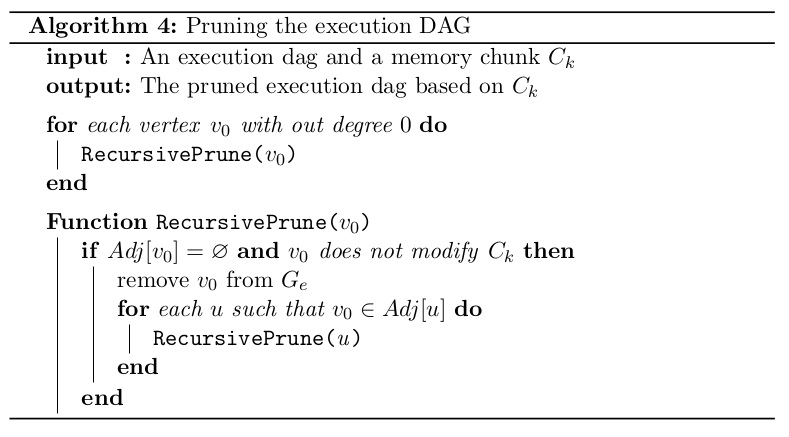
\includegraphics[width=17cm]{../img/Alg4s.png}
\begin{algorithm}
    \DontPrintSemicolon
    \SetKwData{V}{$v_0$}\SetKwData{Graph}{$G_e$}\SetKwData{Shard}{$Sh_k$}\SetKwData{Txns}{$T$}
    \SetKwFunction{RPrune}{RecursivePrune}
    \SetKwProg{Fn}{Function}{}{}
    \SetKwInOut{Input}{input}\SetKwInOut{Output}{output}
    \Input{An execution dag \Graph and a memory shard \Shard}
    \Output{The pruned execution dag based on \Shard}
    \BlankLine
    \For{each vertex \V with out degree $0$}
    {
        \RPrune{\V}\;
    }
    \BlankLine
    \Fn{\RPrune{\V}}
    {
        \If{$Adj[\V] = \varnothing$ {\bf and} \V does not modify \Shard}
        {
            remove \V from \Graph\;
            \For{each $u$ such that edge $(u,\V)$ was in \Graph}
            {
                \RPrune{u}\;
            }
        }
    }
    \caption{Pruning an execution DAG}\label{alg:prune_dag}
\end{algorithm}

If we choose shards in a way that most transactions only modify memory locations of one shard,
likely many transactions of a block only need to be validated by one voting committee and can be validated in
parallel by different committees.

Because the voting committees are selected by random sampling, by choosing large enough samples we can make sure
that having multiple voting committees will not change the security properties of the Argennon agreement protocol.


If a block receives a "reject" certificate from its committee or does not receive a certificate
after \texttt{certificateTimeOut} period of time, it will be conditionally validated by \textbf{all} validators. If
it does not receive an "accept" certificate, the validators initiate the recovery protocol.




The recovery protocol can recover the functionality
of the Argennon blockchain as long as more than 2/3 of the total stake of the system is controlled by honest users
and any network partition resolves after a finite amount of time. The recovery protocol uses two main emergency
procedures to recover the : emergency forking and emergency agreement protocol.

\subsubsection{Emergency Forking}

The reserve committee of delegates can fork the Argennon blockchain, if it gets a valid fork request from
the validators. A valid fork request at
block $b$ is a signature issued by at least $0.8$ of the total \texttt{online} stake
of the validators. The stake values are calculated based on the staking database at block $b - 1$.

For forking at block $b$, the reserve committee of delegates
makes a special fork block which only contains a valid fork request at block $b$, and its parent block is block $b$.
The fork block needs a valid certificate from all $m$ validator committees in order to be valid. A valid fork block
will force the fork, in the sense that any validator receiving it considers the forked chain as the new valid chain.

A validator will issue
an "accept" certificate for a fork block at position $b + 1$ if
\begin{itemize}
    \item the fork block is signed by the reserve committee of delegates.
    \item the fork block contains a valid fork request at block $b$ and block $b$ is its parent.
    \item the validator has not issued a certificate for any block $\geq b + 2$.
    \item the validator has not seen a certificate of validators for any block $\geq b + 2$.
\end{itemize}

Emergency forking may discard at max one block with a valid validator's certificate
from the blockchain, in the worst case scenario.

\subsubsection{Emergency Agreement Protocol}

Emergency agreement protocol is a protocol for deciding between a set of proposals when no committee of
delegates is available. For initiating the protocol, a validator signs a message containing
the hash of a block which will the stake values during voting rounds will be calculated based on its
staking database. A validator starts the protocol if he
receives a message containing a valid block signed by more than 2/3 of the total stake of the validators.
if the block is too old the validator will not enter the agreement protocol.

Emergency agreement is done by voting in rounds. Each round lasts for approximately $\lambda$ units of time.
Users cast two type of votes: \emph{$i$-votes}, which are votes that are valid only in round $i$,
and \emph{final-votes}, which are votes that are valid in any round. A user executes the
following procedure in round $r$ of the voting phase:
\begin{itemize}
    \item if the user has not yet final-voted any value or if $r\mod k = 1$ he $r$-votes a desired proposal
    \item if he sees more than 2/3 round $r$-votes for a proposal $p$ he final-votes $p$
    \item if he sees more than 2/3 final-votes for a proposal he goes to the confirmation phase for $p$
    \item if $clock > r \cdot \lambda$ user goes to the round $r + 1$
\end{itemize}

the confirmation phase
\begin{itemize}
    \item user confirm-votes $p$
    \item if he sees more than 2/3 confirm votes for $p$ he selects $p$ and ends the agreement protocol
    \item if $clock > k \cdot \lambda$ user goes to the round $k + 1$ of voting
\end{itemize}

\subsubsection{Initiating the Recovery Protocol}

A validator will try to initiate the recovery protocol in two situations: when he does not receive any blocks for
\texttt{blockTimeOut} amount of time, or when he sees an evidence which proves the delegates are malicious.

When a validator is not receiving any blocks, first he switches his network to censorship resilient mode. If still he
does not receive any new blocks, he will start validating all the blocks in his blockchain that does not have
a validators' certificate. After he successfully validates the last block, if still he does not receive any blocks,
he will sign and broadcast an \textbf{emergency fork request} message at the last block he has
verified.

If the reserve committee of delegates is already active or If a validator sees a fork request signed
by 2/3 of the total stake of the validators, but does not receive the fork
block after a certain amount of time he will sign and broadcast a request for
emergency agreement on a new reserve committee. the validator puts the last valid block of his
blockchain in the request.

If a validator sees an evidence that proves the delegates are behaving maliciously, he signs and broadcasts a
fork request at approprate block. if the reserve committee is generating blocks he signs a agreement for choosing
a new reserve committee of delegates.

A validator finds a block that conditionally is not valid. in this case validators start validating previous blocks of the
invalid block that does not have a validators' certificate. then the validator sign a fork request at the last valid
block before the invalid block.
the block depends on the specific evidence
recieving a malformed block signed by the delegates for example a block which does not contain all the required feilds

two different blocks signed by the delegates at the same height (same block number)
a block signed by the delegates which is not conditionlly valid and its previous block has a valid certificate from the validators commitee



time out in receiving validators certificate

time out in receiving a new block

finds an invalid block in his blockchain

Online stake goes too low


The delegates stop generating blocks


\paragraph{The delegates fork the blockchain}
%
%Validators stop issuing certificates for normal blocks and they will only issue certificates for \emph{statuts} blocks.
%A status block is a special block which can only contain status change transactions. Status blocks need to be
%certified by all the validators.
%all online validators will check the
%validity of that block. if they do not issue a certificate for that black either